% !TeX spellcheck = en_US
% !TeX root = ./0_article.tex

\section{How to perform BBI in a better way}
	\IEEEPARstart{T}{his} section is dedicated in presenting the various improvements which can be brought to a BBI platform to increase experiments repeatability and reliability.
	\subsection{BBI platforms in the state of the art}
		In the first place, we will analyze, from a theoretical perspective, a typical BBI platform.
		To do so, we created simple platform models allowing to highlight the major limiting factors of such platforms.
		% !TeX spellcheck = en_US
% !TeX root = ./0_article.tex

\begin{figure}[h]
	\centering
	\subfloat[][Typical]{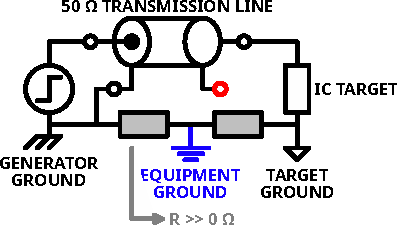
\includegraphics[width=0.5\columnwidth]{./figures/state-of-the-art-platform.pdf}}
	\subfloat[][Improved]{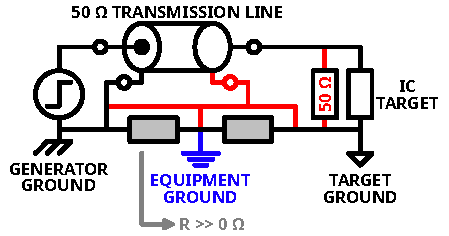
\includegraphics[width=0.5\columnwidth]{./figures/s-bbi-better.pdf}}
	\caption{Simple models of a typical (a) and an improved (b) BBI setup.}
	\label{bbi_setups}
\end{figure}

		The typical platform model is described in Fig. \ref{bbi_setups}.a and shows the main components making a BBI platform such as:
		\begin{itemize}
			\item The voltage pulse generator;
			\item The transmission line;
			\item The grounding installation;
			\item The IC target.
		\end{itemize}
		In addition to this, the schematic shows some important flaws we are going to address.

		While this is not always the case, voltage pulse generators are typically specified to be loaded with a 50 \textOmega\ load, or more generally with a fixed load.
		When performing BBI, the backside of the IC is electrically connected to the generator output.
		Therefore, outside of luck alone, it is very rare that the impedance presented by the IC to the generator perfectly matches the required one.
		It implies that the generator will be, most of the time, out of specifications, and that the conditions will vary depending on the chosen IC and the location of the BBI probe.
		This can lead to issues such as errors in the set-point voltage and pulse width, and ringing in the transmission line.
		It then represents a first flaw to the typical approach.

		Then, there is the grounding installation.
		The model presents a non-ideal but simple platform grounding.
		The reference, used by the oscilloscope and the main computer, is represented in blue and called "equipment ground".
		Ideally, every ground on the platform is connected to this reference with a very low impedance interconnection.
		However, depending on the hardware used, it may greatly vary from one platform to another.
		In the model, the secondaries generator and target grounds are connected to the reference thanks to vastly imperfect interconnections, whose impedance is significantly higher than zero.
		This mainly lead to set-point errors due to shifts in the voltage pulse amplitude.
		Therefore, it limits the inter-platform repeatability of BBI experiments.

	\subsection{Our BBI platform}
		As the commercial platforms, our platform is focused on two main pieces of equipment: a voltage pulse generator and a metallic probe.
		
		The generator model is the AVRK-4-B from the society Avtech Electrosystems Ltd.
		This model is commonly used for EMFI, but is suitable for BBI, and its specifications are the following:
		\begin{itemize}
			\item Pulse amplitude: \textpm\ [150, 750] V;
			\item Pulse width: [6, 20] ns;
			\item First edge rise/fall time: 4 ns;
			\item Second edge rise/fall time: load dependent;
			\item Recovery time: \textless\ 1 ms;
			\item Propagation delay (PD): 150 ns;
			\item Jitter: \textpm\ 100 ps \textpm\ 0.03 \% of PD;
			\item DC-coupled output;
			\item Loaded with 50 \textOmega.
		\end{itemize}
		% !TeX spellcheck = en_US
% !TeX root = ./0_article.tex

\begin{figure}
	\centering
	\subfloat[][Global view]{\includegraphics[width=0.4\columnwidth]{./figures/sondeBBI_loin_raw.png}}
	\hspace{0.1\columnwidth}
	\subfloat[][Zoomed view]{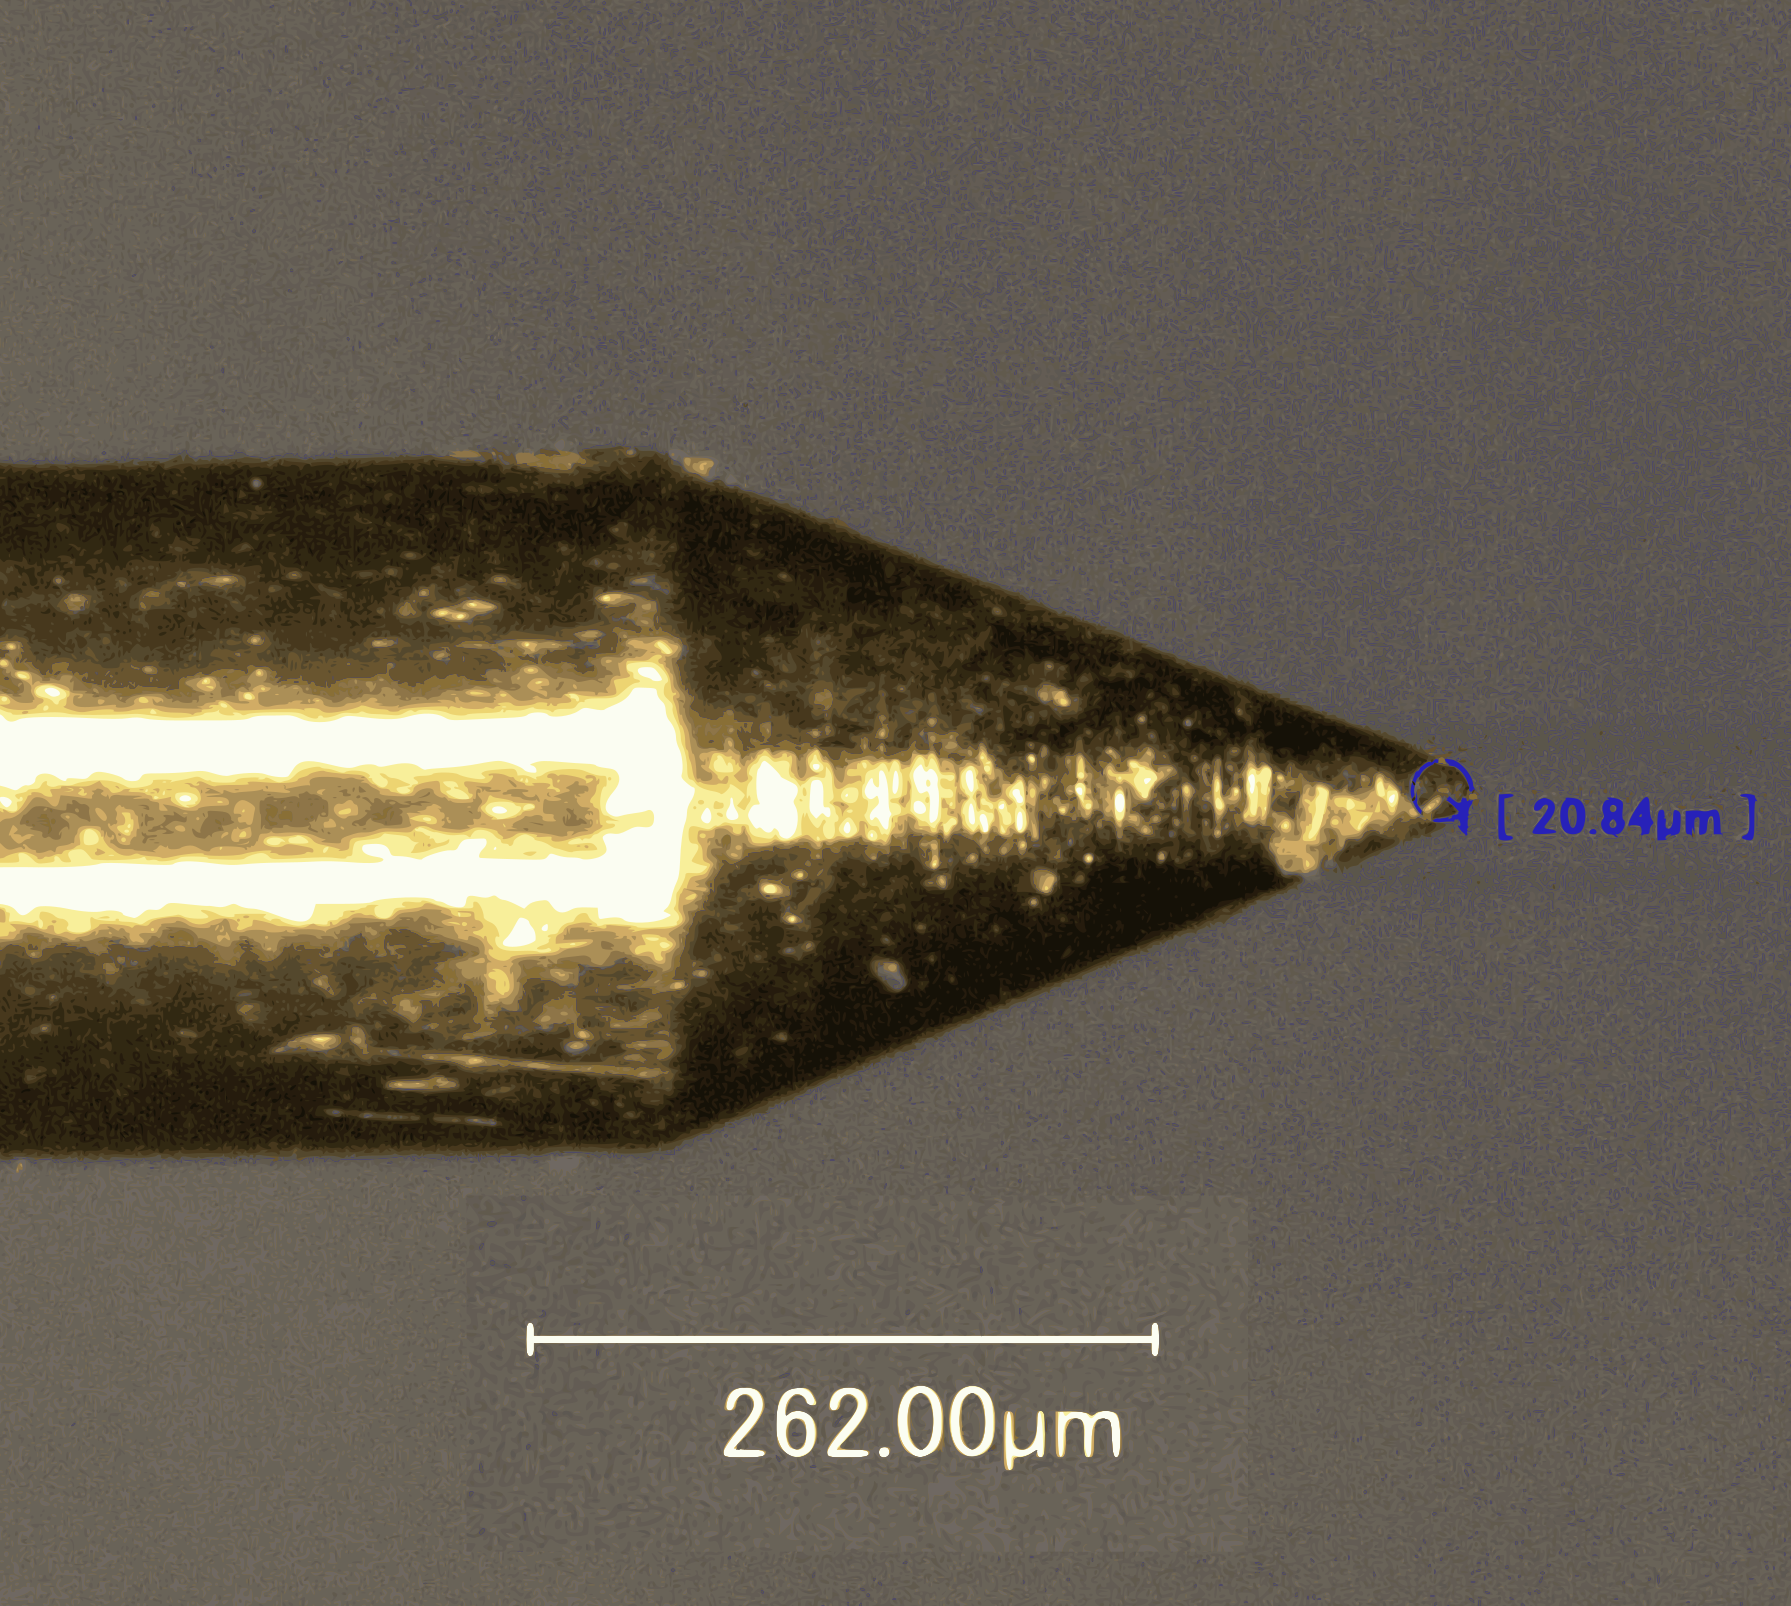
\includegraphics[width=0.4\columnwidth]{./figures/pointeBBI2.png}}
	\caption{Our custom BBI probe.}
	\label{bbi_probe}
\end{figure}
		Probably the most distinctive piece of equipment when it comes top BBI is the probe.
		Some BBI probes can be active, others passive and less expensive.
		However, it is important to keep this piece of equipment relatively cheap as it endures most of the physical strain on a BBI platform, and should be easy to replace or repair.
		Fig. \ref{bbi_probe} shows two pictures of our probe from different angles.
		The one we use is custom made around three parts:
		\begin{itemize}
			\item A spring-loaded metallic tip, with a 20 \textmu m head diameter;
			\item A SMA connector, where the tip is soldered;
			\item A custom 3D-printed enclosure holding the pieces together and cheap to replace.
		\end{itemize}
		The spring-loaded tip is 17 mm long and has a global diameter of 0.635 mm.
		It is specified for a 1.5 A nominal current, and its electrical resistance measures around 70 m\textOmega.
		The total cost of the probe is of 20 \texteuro.

	\subsection{Improvements proposed}
		To circumvent the previously introduced limitations, we propose two corrections to generalize the platforms and improve the repeatability.

		First, let us talk about the improper grounding,
		Alleviating this issue is fairly straightforward.
		To do so, we propose to choose a reference, such as the equipment ground, and bypass all the grounds with low-impedance interconnections from this reference, as proposed in red in Fig. \ref{bbi_setups}.b.

		Then, concerning the impedance mismatch of the generator, multiple solutions can be approached.
		The best solution would be to implement an adaptive impedance matching system with active feedback, able to measure in real-time the impedance seen by the generator.
		However, adopting such a method is costly and long to set up in comparison to the next solution.
		Therefore, we propose a much simpler approach.
		Since, most of the time, the impedance presented by the IC on its backside is in the order of 1 k\textOmega\, approaching the 50 \textOmega\ expected by the generator can be done by connecting in parallel to the IC a 50 \textOmega\ resistor, as it is shown in the schematic in Fig. \ref{bbi_setups}.b.

	\subsection{Platform improvements in practice}
		% !TeX spellcheck = en_US
% !TeX root = ./0_article.tex

\begin{figure}[h]
	\centering
%	\subfloat[][Typical]{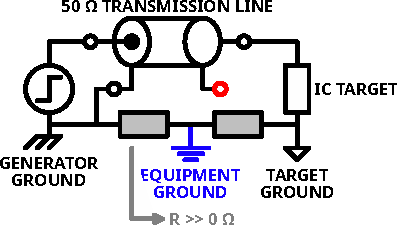
\includegraphics[width=0.5\columnwidth]{./figures/state-of-the-art-platform.pdf}}
%	\subfloat[][Improved]{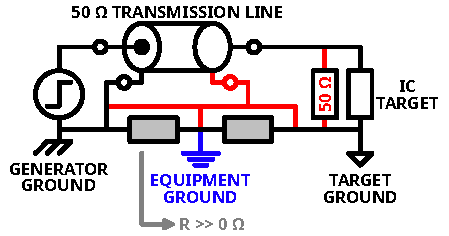
\includegraphics[width=0.5\columnwidth]{./figures/s-bbi-better.pdf}}
	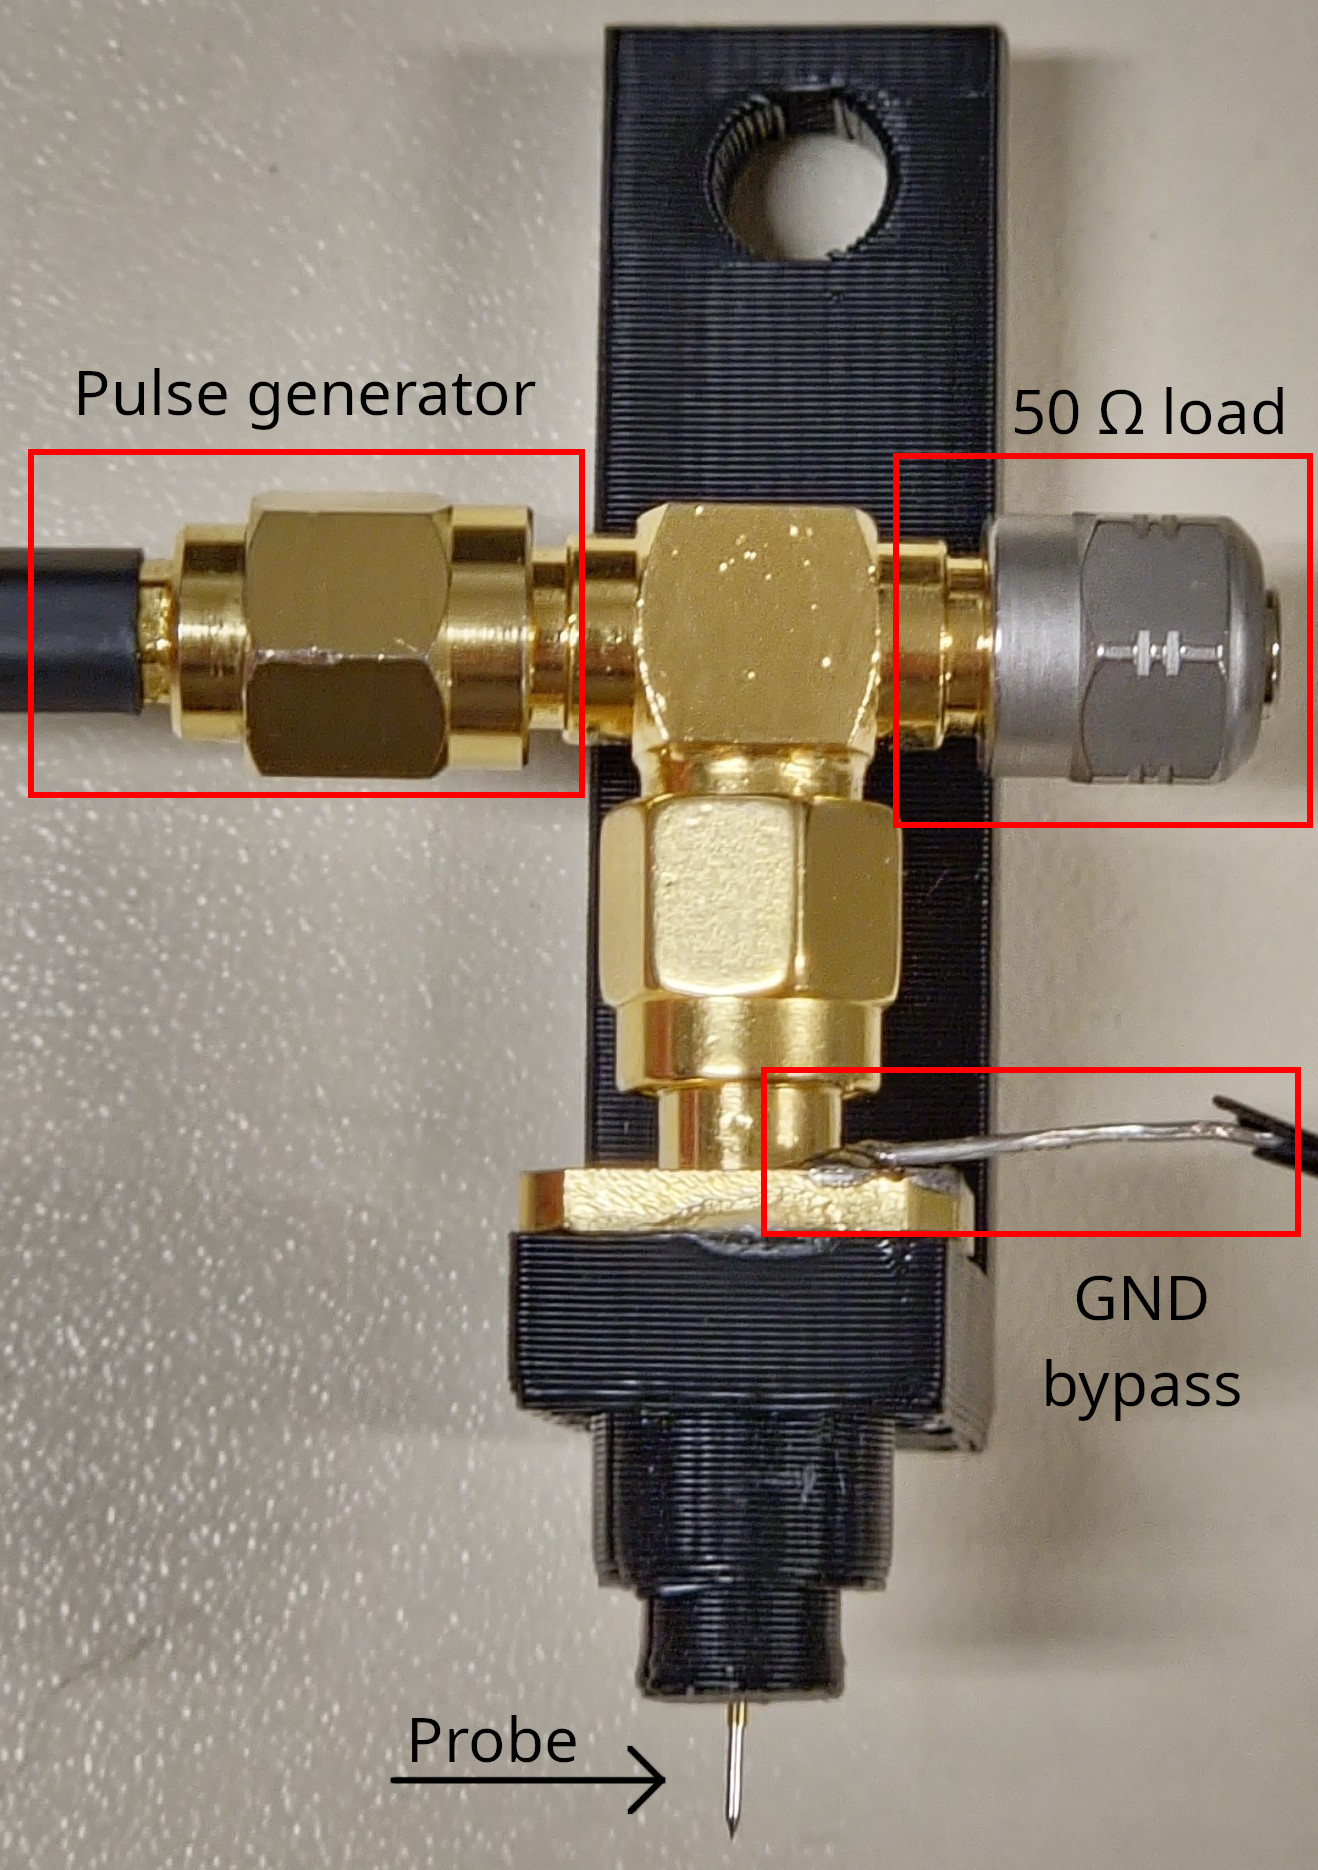
\includegraphics[width=0.40\columnwidth]{./figures/sondeGndSource.jpg}
	\caption{Impedance matching in practice.}
	\label{imp_match_real}
\end{figure}

		The proposed solution concerning the approximate impedance matching is shown in Fig. \ref{imp_match_real}.
		The picture shows the BBI probe with a compensation load connected in parallel.
		To show the actual interests of these improvements, let us analyze signals from an actual platform.

		We will compare before and after results and analyze the differences made by these improvements.
		To that end, we set up simple experiments consisting in injecting a voltage pulse into our IC target, measuring the voltage pulse at the probe and the current in the IC.
		% !TeX spellcheck = en_US
% !TeX root = ./0_article.tex

\begin{figure}[h]
	\centering
	%	\subfloat[][Typical]{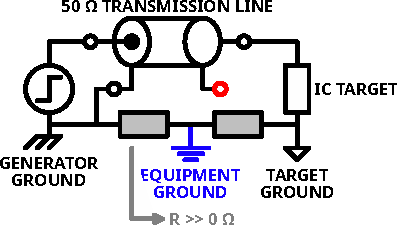
\includegraphics[width=0.5\columnwidth]{./figures/state-of-the-art-platform.pdf}}
	%	\subfloat[][Improved]{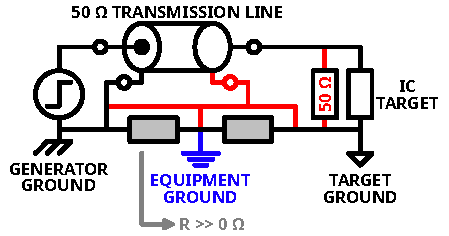
\includegraphics[width=0.5\columnwidth]{./figures/s-bbi-better.pdf}}
	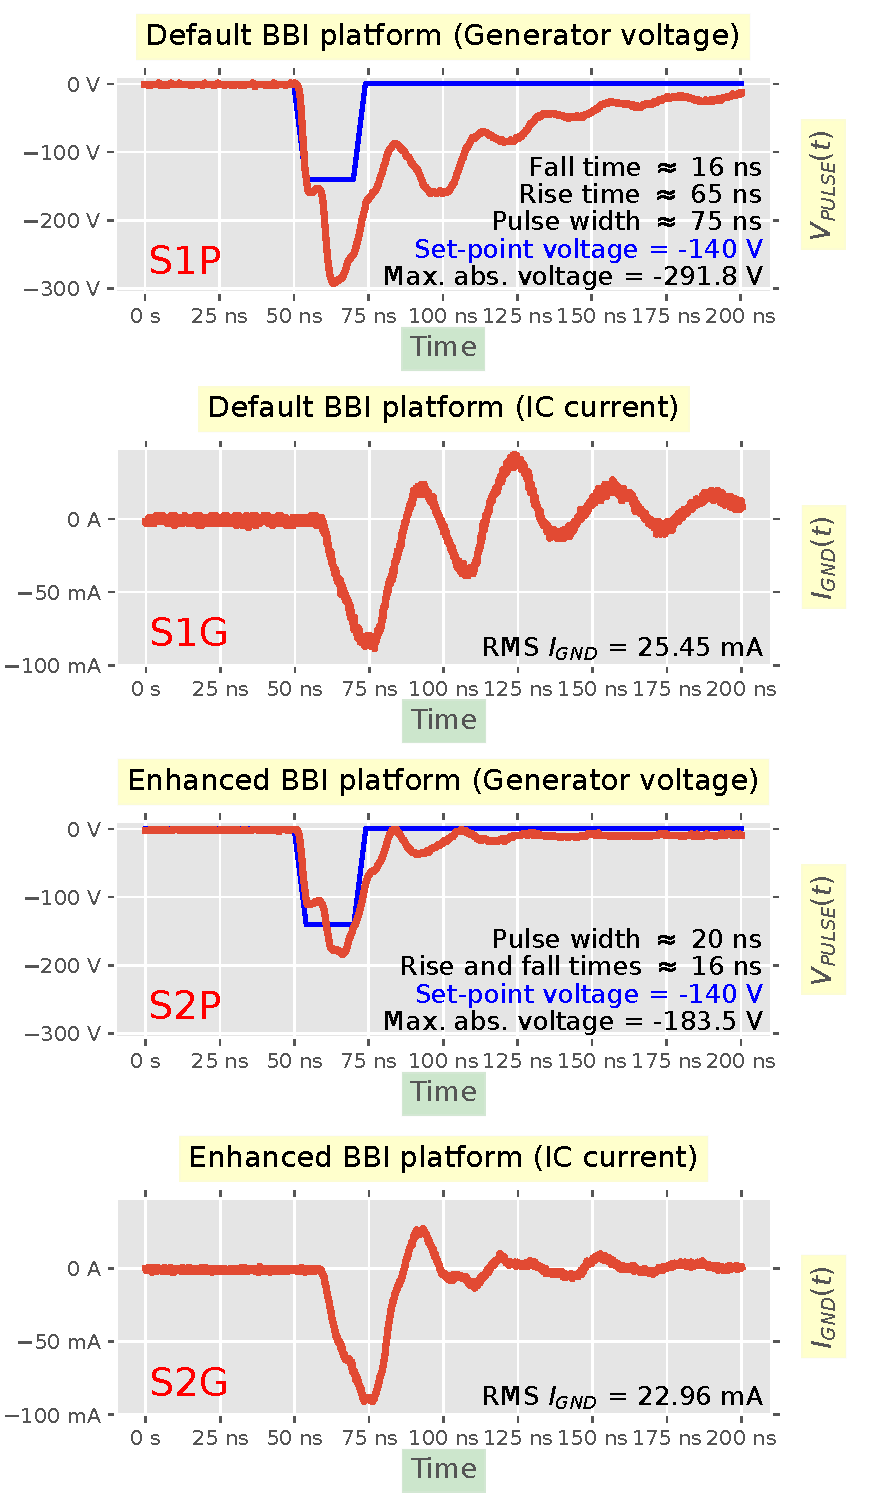
\includegraphics[width=\columnwidth]{./figures/realPulsesComparisons.pdf}
	\caption{Platform improvements in practice}
	\label{actual_imp}
\end{figure}

		Fig. \ref{actual_imp} presents the waveform results of such experiments.
		The figure is split in two main parts, the top row shows the results before the improvements, and the bottom row shows the results after the improvements.
		The experimental conditions are the following:
		\begin{itemize}
			\item Voltage pulse amplitude = -140 V;
			\item Voltage pulse width = 20 ns;
			\item Rise and fall times = 4 ns.
		\end{itemize}

		The waveform S1P shows in blue the ideal waveform according to the generator settings and in red the measured waveform.
		In addition to this are annotated some noteworthy values.
		The first thing to notice here is the obvious undershoot of about -110 \% under the set-point.
		It is far from being desirable when performing fault injection as the voltage amplitude is of great importance when considering the method effects on the IC.
		Furthermore, the pulse width is 275 \& higher than the set-point, measuring 75 ns instead of 20 ns.
		It is an additional issue as it annihilates the accuracy needed in this context, and leads to longer pulses injected into the IC and potentially more energy than required.
		Additionally, the rise and fall times are also 4 to 16 times higher than expected.
		Eventually, we can notice damped oscillations, probably the proof of ringing in the transmission line.

		Then, the waveform S1G, associated with the previous one, shows the IC ground current.
		Here, the damped oscillations are more clearly visible, in addition to the much longer than expected pulse duration.
		The RMS value of the injected current measures around 25 mA.

		Afterwards, the waveform S2P shows the results with the proposed improvements
		The voltage pulse amplitude is much closer to the set-point, with an undershoot of -31 \%.
		It is not perfect, but considering the simple nature of the impedance matching we propose, it was to be expected.
		On another note, the pulse width set-point is perfectly respected.
		However, the rise and fall times are still 4 times higher.
		Then, when looking at the S2G current waveform, we can remark the ringing reduction, while the amount of transferred energy remains approximately the same.

	\subsection{Further platform improvements comparison}
		To be able to illustrate further the actual interests of the proposed improvements, we did not only set up electrical measurements, but a complete differential fault attack (DFA).
		Indeed, performing fault injection is mainly used to perform attacks, therefore it makes sense to verify the soundness of the improvements in this context.
		We chose to perform a single bit DFA ou our IC target.
		The target embeds a dedicated cryptographic core, which we set up using a 128 bits AES.
		We then decided to perform the Giraud's DFA \cite{giraudDfa}, originally described in 2002.
		This attack requires creating single bit faults in one or more bytes on the targeted AES.
		Our target was clocked at 40 MHz thanks to an external 8 MHz crystal, and powered with 3.3 V for the experiment.

		\subsubsection{Preliminary experiments}
			Before setting up the attack, we had to set up experiments allowing us to find the optimal locations in the AES sub-circuit where the attack could be performed.
			To do so, we created what we call Fault Analysis Mappings (FAM).
			These experiments consist in creating maps of a specific region of the IC, in that case the AES sub-circuit, and analyzing the IC behavior while performing BBI.
			The behavior is split into seven cases:
			\begin{itemize}
				\item Correct: the AES responds normally;
				\item Monobit Monobyte fault;
				\item Multibit Monobyte faults;
				\item Monobit Multibyte faults;
				\item Multibit Multibyte faults;
				\item Crash: the circuit did not respond correctly;
				\item Timeout: the circuit did not respond.
			\end{itemize}
			Therefore, as we need single bit faults, only two cases are valid for the Giraud's DFA.
			To be able to compare the two platforms, we performed a FAM on each one of them, using the following parameters:
			\begin{itemize}
				\item Pulse amplitude: from -150 V to -400 V with -5 V steps;
				\item Pulse width = 4.5 ns;
				\item Pulse delay of 150 ns + 553 ns targeting the penultimate AES round;
				\item A 40 mm displacement step.
			\end{itemize}
			Depending on the IC behavior, the experiments cant take up to 36 hours.
			The parameters were chosen to minimize the maximum energy transferred into the IC to avoid damaging it as much as possible.
			% !TeX spellcheck = en_US
% !TeX root = ./0_article.tex

\begin{figure}[h]
	\centering
%		\subfloat[][Typical]{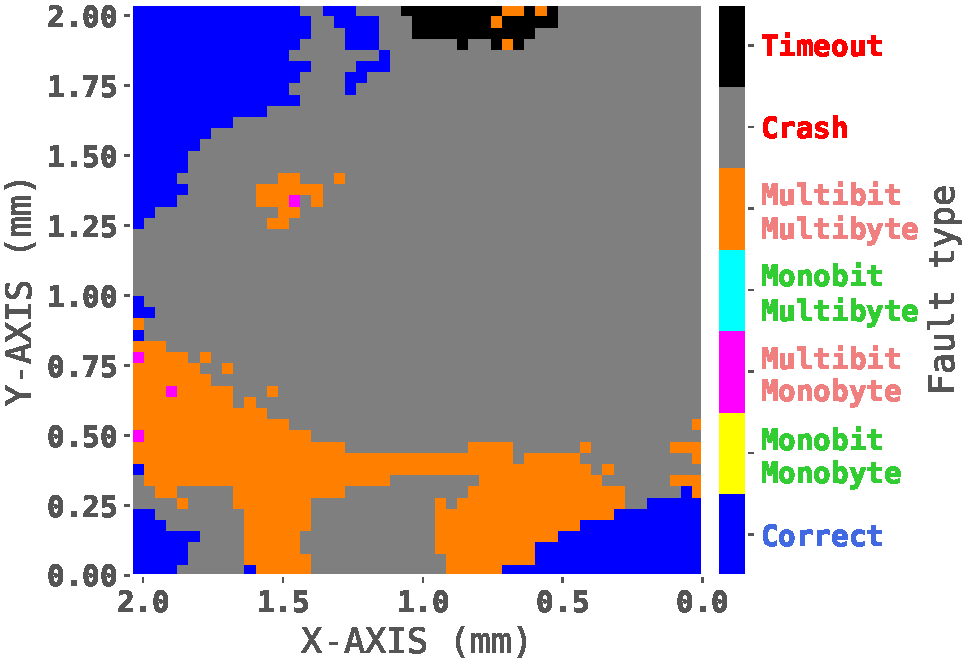
\includegraphics[width=0.5\columnwidth]{./figures/aesFastGndOnly-cropped.pdf}}
%		\subfloat[][Improved]{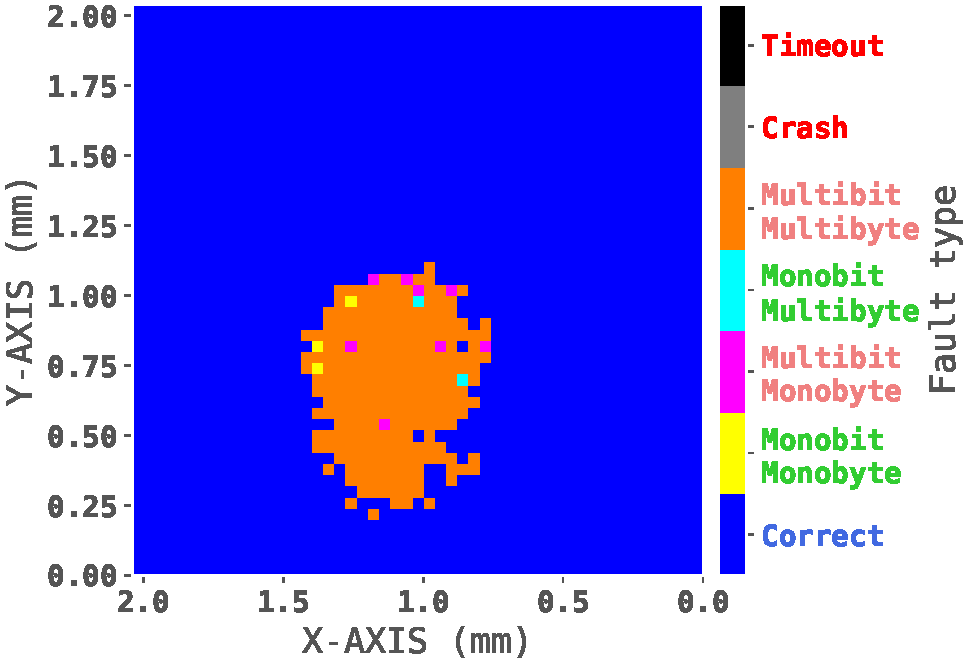
\includegraphics[width=0.5\columnwidth]{./figures/aesFastImpGnd-cropped.pdf}}
		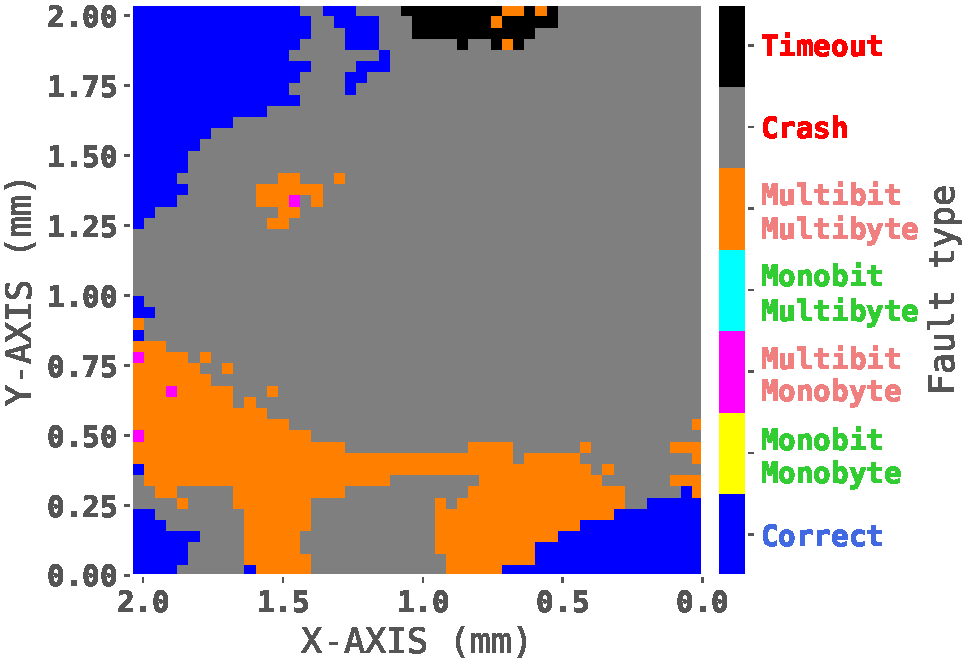
\includegraphics[width=0.995\columnwidth]{./figures/aesFastGndOnly-cropped.pdf}
		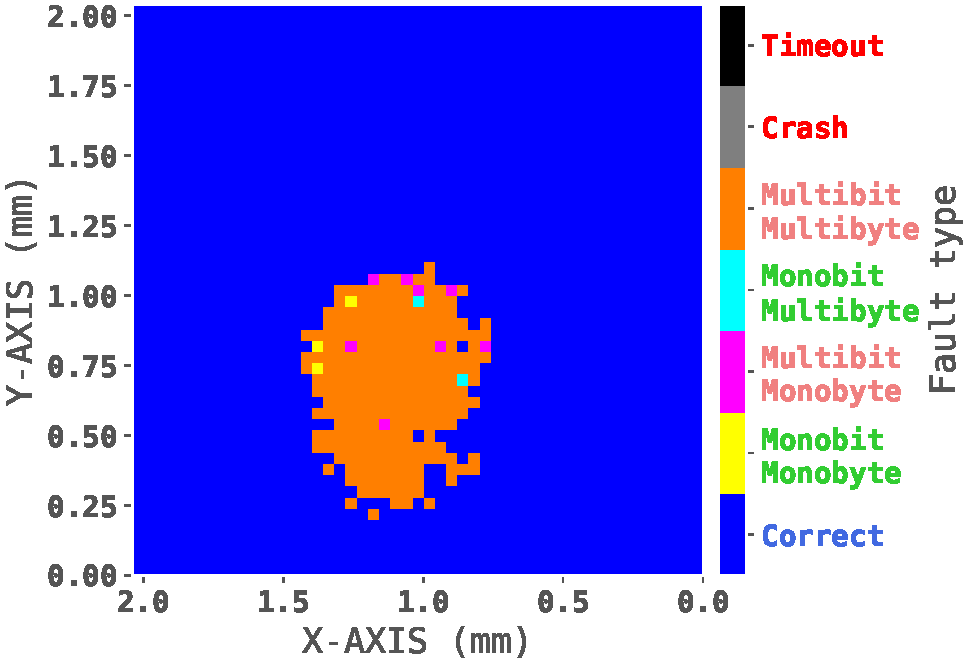
\includegraphics[width=1.0\columnwidth]{./figures/aesFastImpGnd-cropped.pdf}
	\caption{Giraud's attack preliminary FAM}
	\label{giraud_fam}
\end{figure}

			Fig. \ref{giraud_fam} presents the FAM results for both a typical and an improved platform.
			The mapped area encloses a little more than the actual AES, to be sure to map its entirety.

			Let us look at Fig. \ref{giraud_fam}.a first.
			What is interesting here is that we can spot numerous location where the circuit crashed.
			More specifically, they represent 70 \% of the mapped area.
			This behavior is problematic in such an experiment as it cannot lead to any useful data for a DFA.
			Despite trying various experimental parameters, we could not observe single bit faults using this setup.
			However, multibit multibyte faults were easily observed, which was to be expected as they are easy to perform without much effort.

			Then, let us discuss Fig. \ref{giraud_fam}.b.
			The first interesting thing to remark is the total absence of IC crash.
			It is a desirable behavior as it indicates that we did not set a too high voltage pulse.
			Then, concerning monobit faults, we can spot five locations.
			It is a good sign for a preliminary experiment as it indicates the feasibility of such faults.
			It does not mean that we can perform the attack on one location.
			However, it means that we can use these locations as good starting points to perform the DFA.

		\subsubsection{DFA results}
			To perform the DFA, we focused on the five previously found monobit locations above the AES core.
			Then, for each location, we used the following parameters:
			\begin{itemize}
				\item Voltage ranging from -300 V to -600 V;
				\item Pulse width ranging from 4.5 ns to 5.5 ns;
				\item Injection delay ranging from \textpm 10 ns around the penultimate AES round.
			\end{itemize}
			For each set of experimental settings, we had to set some limits when trying to inject faults.
			Indeed, it is required to create a finite experiment.
			The first limit consists in trying to retrieve a maximum of 100 single bit fault.
			Then, and because it cannot be achieved for every set of parameters, we set another limit of 10000 tries to achieve the previous limit.
			% !TeX spellcheck = en_US
% !TeX root = ./0_article.tex

\begin{table*}[ht]
	\centering
	\begin{tabularx}{\textwidth}{XXXXXXXXXXXXXXXXX}
		\#B & 0 & 1 & 2 & 3 & 4 & 5 & 6 & 7 & 8 & 9 & 10 & 11 & 12 & 13 & 14 & 15 \\ \hline
		K10 & 0xFF & 0x1F & \cellcolor{red!25}0x42 & 0xE8 & 0xEF & \cellcolor{red!25}0x44 & 0xA5 & 0x6A & 0xCA & 0xE7 & 0x55 & 0x3C & 0xFD & 0x65 & 0x39 & 0x26 \\
		KEY & 0x01 & 0x23 & 0x45 & 0x67 & 0x89 & 0xAB & 0xCD & 0xEF & 0xDE & 0xAD & 0xBE & 0xEF & 0x12 & 0x34 & 0x43 & 0x21
	\end{tabularx}
	\caption{Giraud DFA}
	\label{table_giraud}
\end{table*}

			Thanks to this, we retrieved, using the five locations, 14 out of 16 bytes of the AES secret key, as shown in Table \ref{table_giraud}.
			The red cells indicate the two byes not retrieved thanks to the Giraud's DFA.
			To retrieve these last two bytes, we used a brute force method.
			Considering a slow laptop being able to compute approximately $10 \cdot 10^3$ AES encryptions per second, the 16 remaining bits representing 65536 combinations, we decided to blindly calculate every possibility.
			That represents around 6.5 seconds of total computation.

%	Three main flaws lie in the platform in its current state:
%	\begin{itemize}
%		\item The pulse generator
%	\end{itemize}
